\documentclass[../main.tex]{subfiles}
\begin{document}
\begin{itemize}
    \item \textbf{grandezze scalari:} $t,T,d,m,f,E,A.V,...$
    \item \textbf{grandezze vettoriali:} $\vec{v}, \vec{a}, \vec{F}, ...$
\end{itemize}

\vspace{1cm}
\begin{center}
    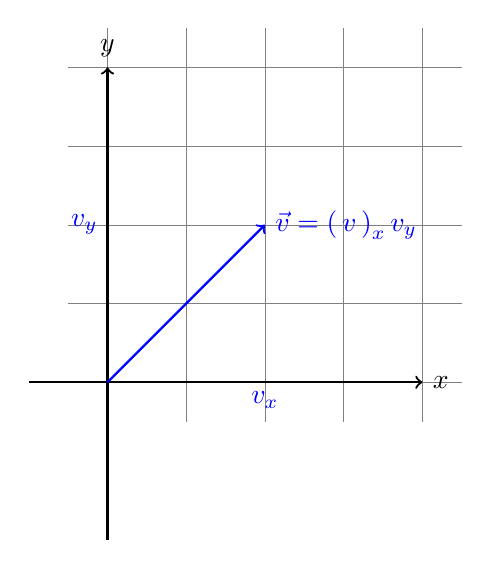
\begin{tikzpicture}
        % Disegna la griglia
        \draw[very thin, gray] (-0.5,-0.5) grid (4.5,4.5);
        
        % Disegna assi
        \draw[thick,->] (-1,0) -- (4,0) node[right] {$x$}; % Asse x
        \draw[thick,->] (0,-2) -- (0,4) node[above] {$y$}; % Asse y

        % Disegna la funzione y = 3x - 2
        \draw[->, domain=-0:2,smooth,variable=\x,blue,thick] 
        plot ({\x},{\x}) node[right] {$\vec{v}=\begin{pmatrix}
            v_x \\
            v_y
        \end{pmatrix}$};

        \node [blue,below] at (2, 0) {$v_x$};
        \node [blue,left] at (0, 2) {$v_y$};
    \end{tikzpicture}
\end{center}

\begin{align*}
    \left\lVert \vec{v}\right\rVert = v =& \sqrt{v_x^2 + v_y^2} \\
    v_x =& v \cdot cos(\alpha) \\
    v_y =& v \cdot sin(\alpha) \\
    v_y =& v_x \cdot tan(\alpha) \\
\end{align*}

Esiste una notazione alternativa, ecco alcuni esempi:
\begin{align*}
    \vec{v} =& \begin{pmatrix}
        3 \\
        6
    \end{pmatrix}
    = 3\hat{x} + 6\hat{y} \text{, $\hat{x}$ e $\hat{y}$ rappresentano dei versori} \\
    \vec{g} =& \begin{pmatrix}
        0 \\
        -9.81
    \end{pmatrix} \frac{m}{s^2}
    =(0\hat{x} - 9.81\hat{y}) \frac{m}{s^2}
\end{align*}

Proprietà utili:
\begin{itemize}
    \item Scomposizione
    \item Somma
    \item Prodotto tra un vettore e uno scalare
\end{itemize}

\end{document}